\documentclass[fleqn,10pt]{wlscirep}
\usepackage[utf8]{inputenc}
\usepackage[T1]{fontenc}
\usepackage[english]{babel}
\usepackage{graphicx}
\usepackage{float}
\usepackage{xcolor}
\usepackage{amsmath}
\usepackage{amsthm}
\usepackage{amssymb}
\usepackage{amsfonts}
\usepackage{bm}

\def\mywarn#1{\textcolor{red}{#1}}
\def\myemph#1{\textcolor{blue}{#1}}
\def\mycell#1{\textcolor{brown}{#1}}

\graphicspath{{figures/}}

% use xelatex (set Tex-engine) can show the bold
% https://tex.stackexchange.com/questions/21200/auctex-and-xetex
\newcommand{\myvec}[1]{\boldsymbol{#1}}
\newcommand{\myset}[1]{\{#1\}}
\newcommand{\mysize}[1]{|#1|}
\newcommand{\mydef}{\triangleq}
\newcommand{\mye}{\mathbb{E}}
\newcommand{\mymucond}{\mu_{c_i}}
\newcommand{\mymuind}{\mu_{b_i}}

\title{MSCC:Multiple-Subject Differential Expression Analysis for
  Single-Cell RNA-Sequencing Data}

%% Notice placement of commas and superscripts and use of &
%% in the author list

% \author{Aauthor$^{1,2}$, Bauthor$^2$ \& LastAuthor$^2$}
\author[1,*]{Songpeng Zu}
\author[2,3 *]{Avinash Das Sahu}
\author[2,3,+]{Xiaole Shirley, Liu}
\author[1,+]{Jun S. Liu}

\affil[1]{Department of Statistics, Harvard University, USA}
\affil[2]{Harvard School of Public Health, Harvard University, USA}
\affil[3]{Dana-Farber Cancer Institute, Boston, USA}
\affil[+]{Corresponding authors}
\affil[*]{These authors contributed equally to this work}

\keywords{Differential analysis, single-cell sequencing, batch effect,
multiple subjects}

\begin{abstract}
A major challenge in single-cell data analysis is cells from the same
sample are not independent(pseudoreplication bias). Commonly used
differential expression methods fail to account for this bias that has lead to
inflated false positives. We still see several genes with extremely small
p-values even when data is permuted suggesting these methods are capturing
signals that are non-biological. We found that several published results
suffer from the bias, which had exacerbated the replicability crisis in the
field. To address this, we are developing a Bayesian approach (MSSC) to
identify differentially expressed genes by accounting pseudoreplication bias
in the model. We have shown our method dramatically decreases the false
positive rate using simulation as well as using real data where ground truth
is known.
\end{abstract}

\begin{document}
\flushbottom
\maketitle
\thispagestyle{empty}
\section*{Introduction}

\section*{Results}
\subsection*{Simulation studies}
\begin{figure}[H]
  \centering
  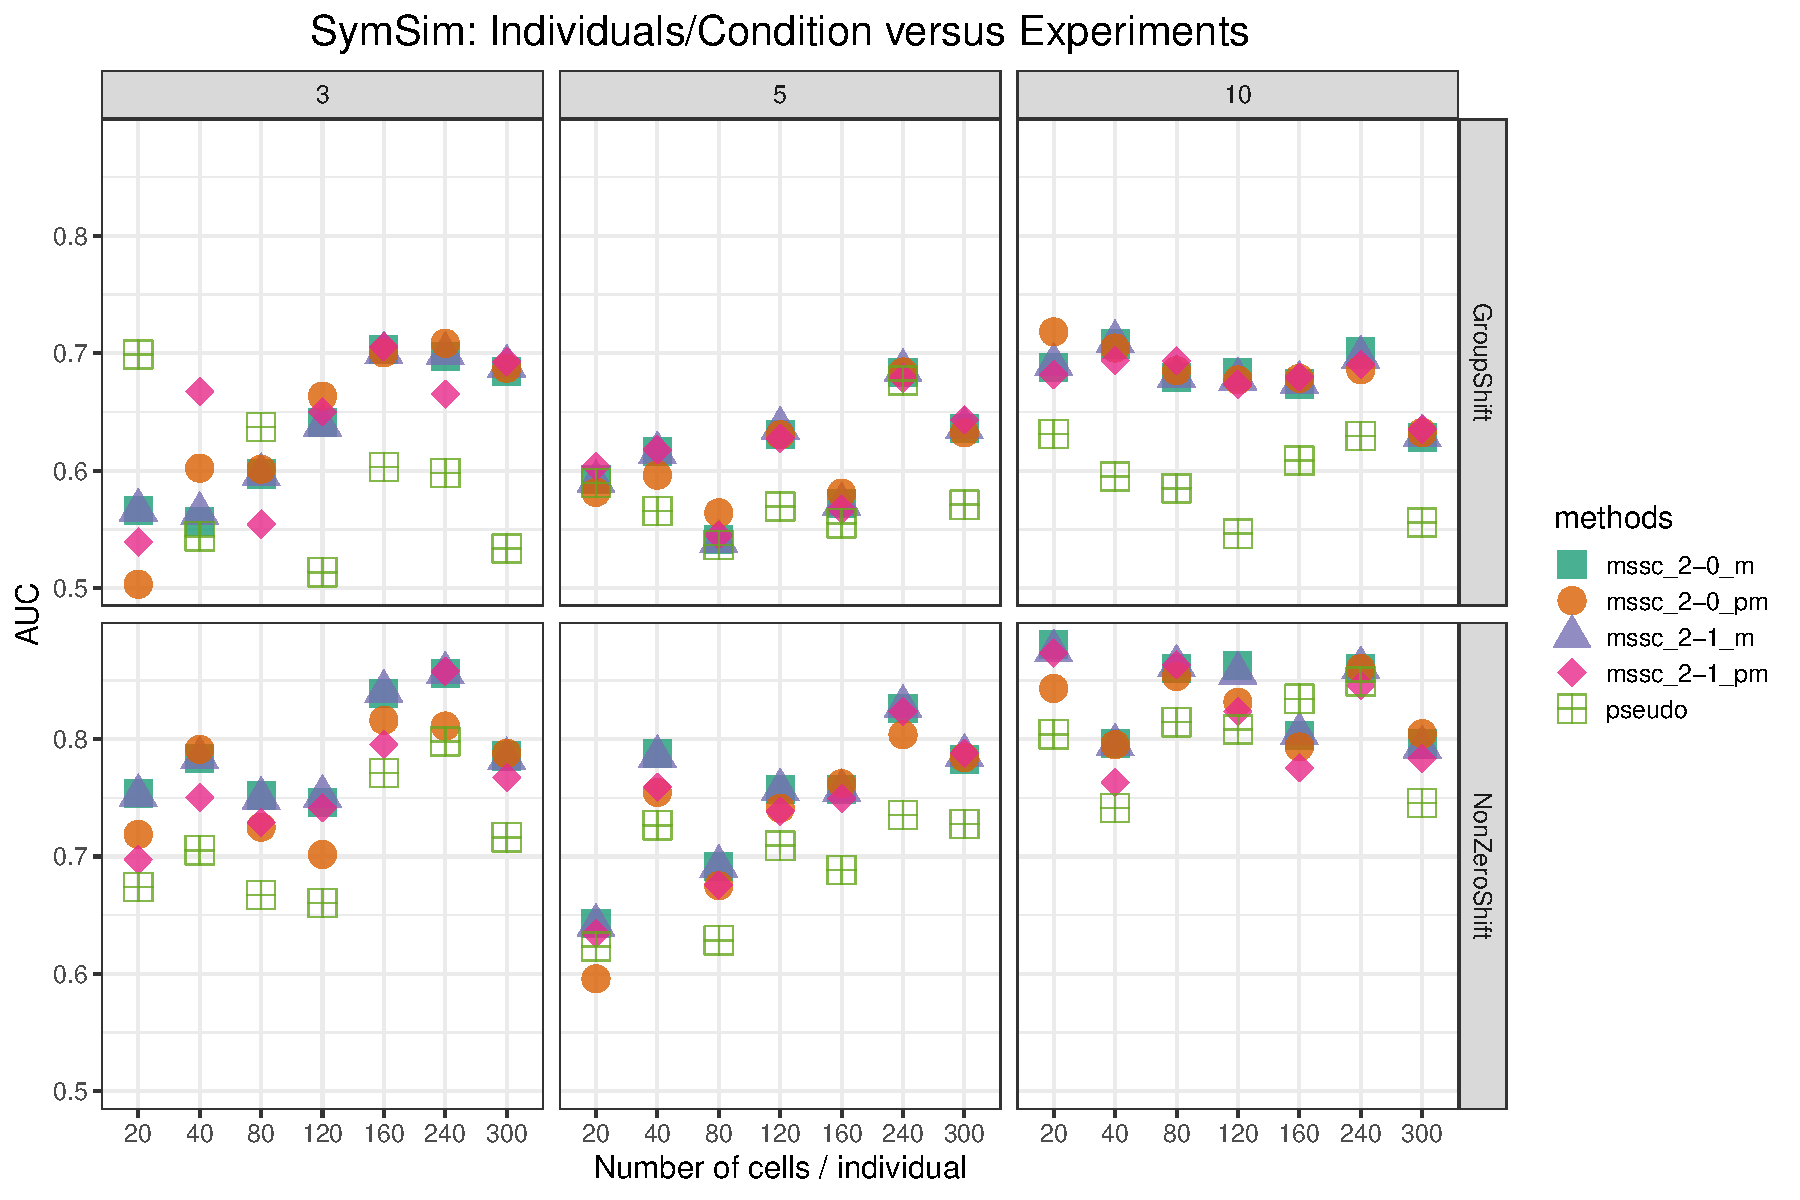
\includegraphics[width=\textwidth]{SymSim_Summarize}
  \caption{SymSim Simulations under different number of individuals.}
\end{figure}
\begin{figure}[H]
  \centering
  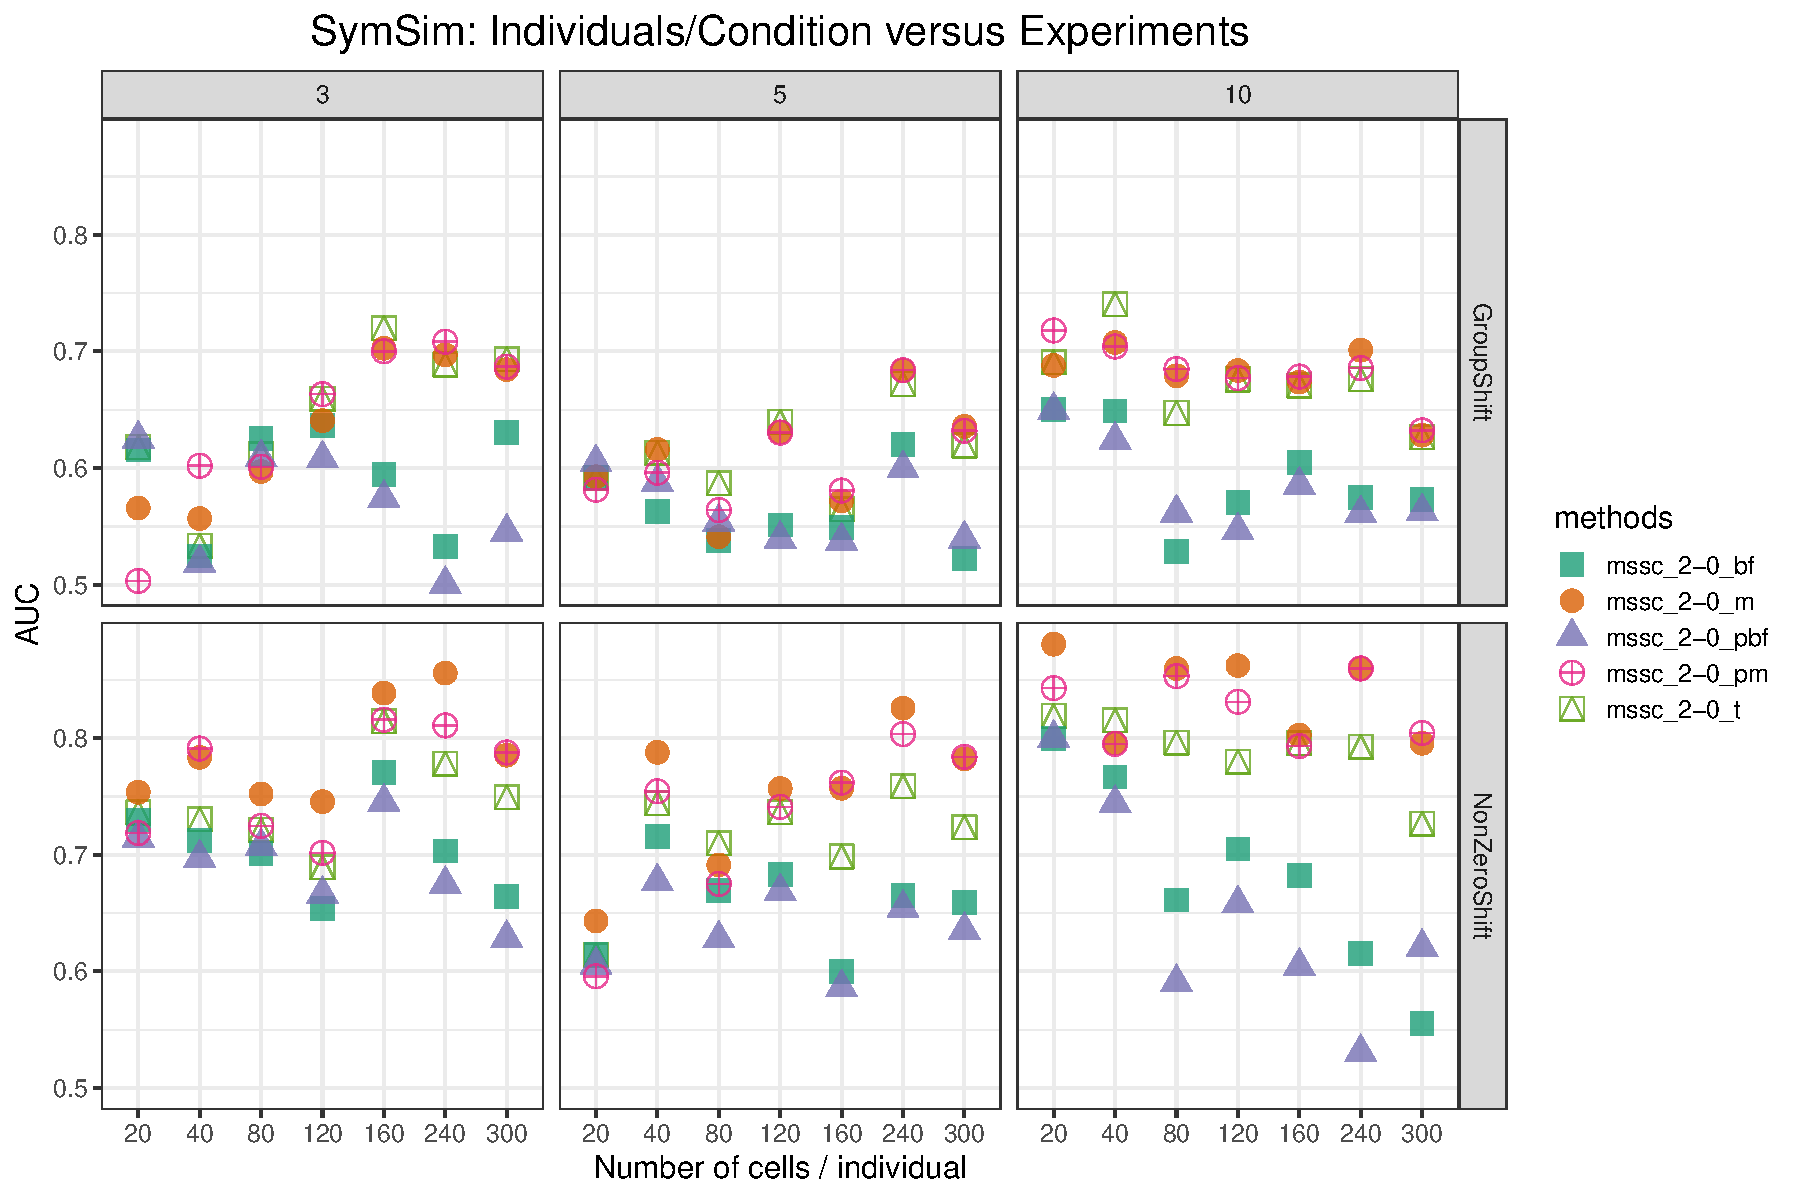
\includegraphics[width=\textwidth]{SymSim_mssc20_Summarize}
  \caption{Supplementary: different measurements in mssc-20.}
\end{figure}
\begin{figure}[H]
  \centering
  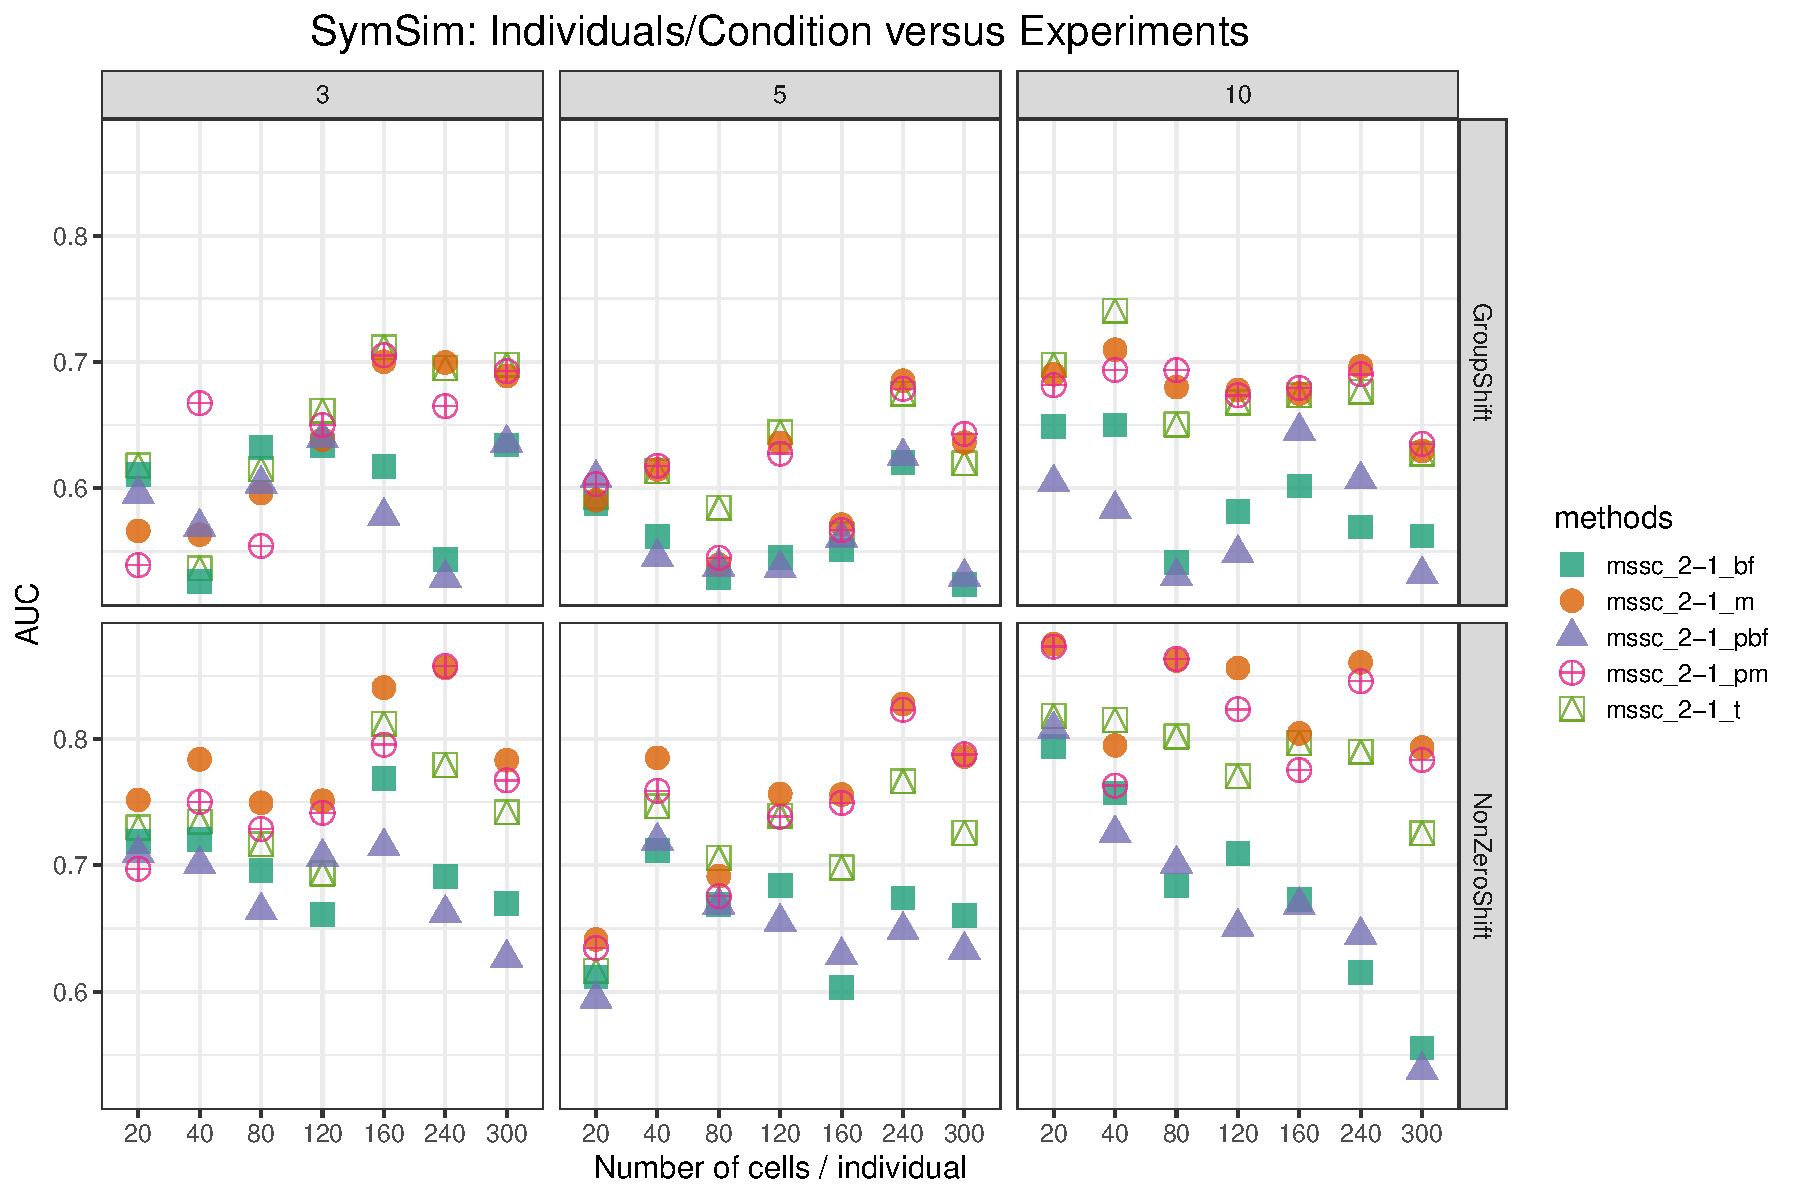
\includegraphics[width=\textwidth]{SymSim_mssc21_Summarize}
  \caption{Supplementary: different measurements in mssc-21.}
\end{figure}

\begin{figure}[H]
  \centering
  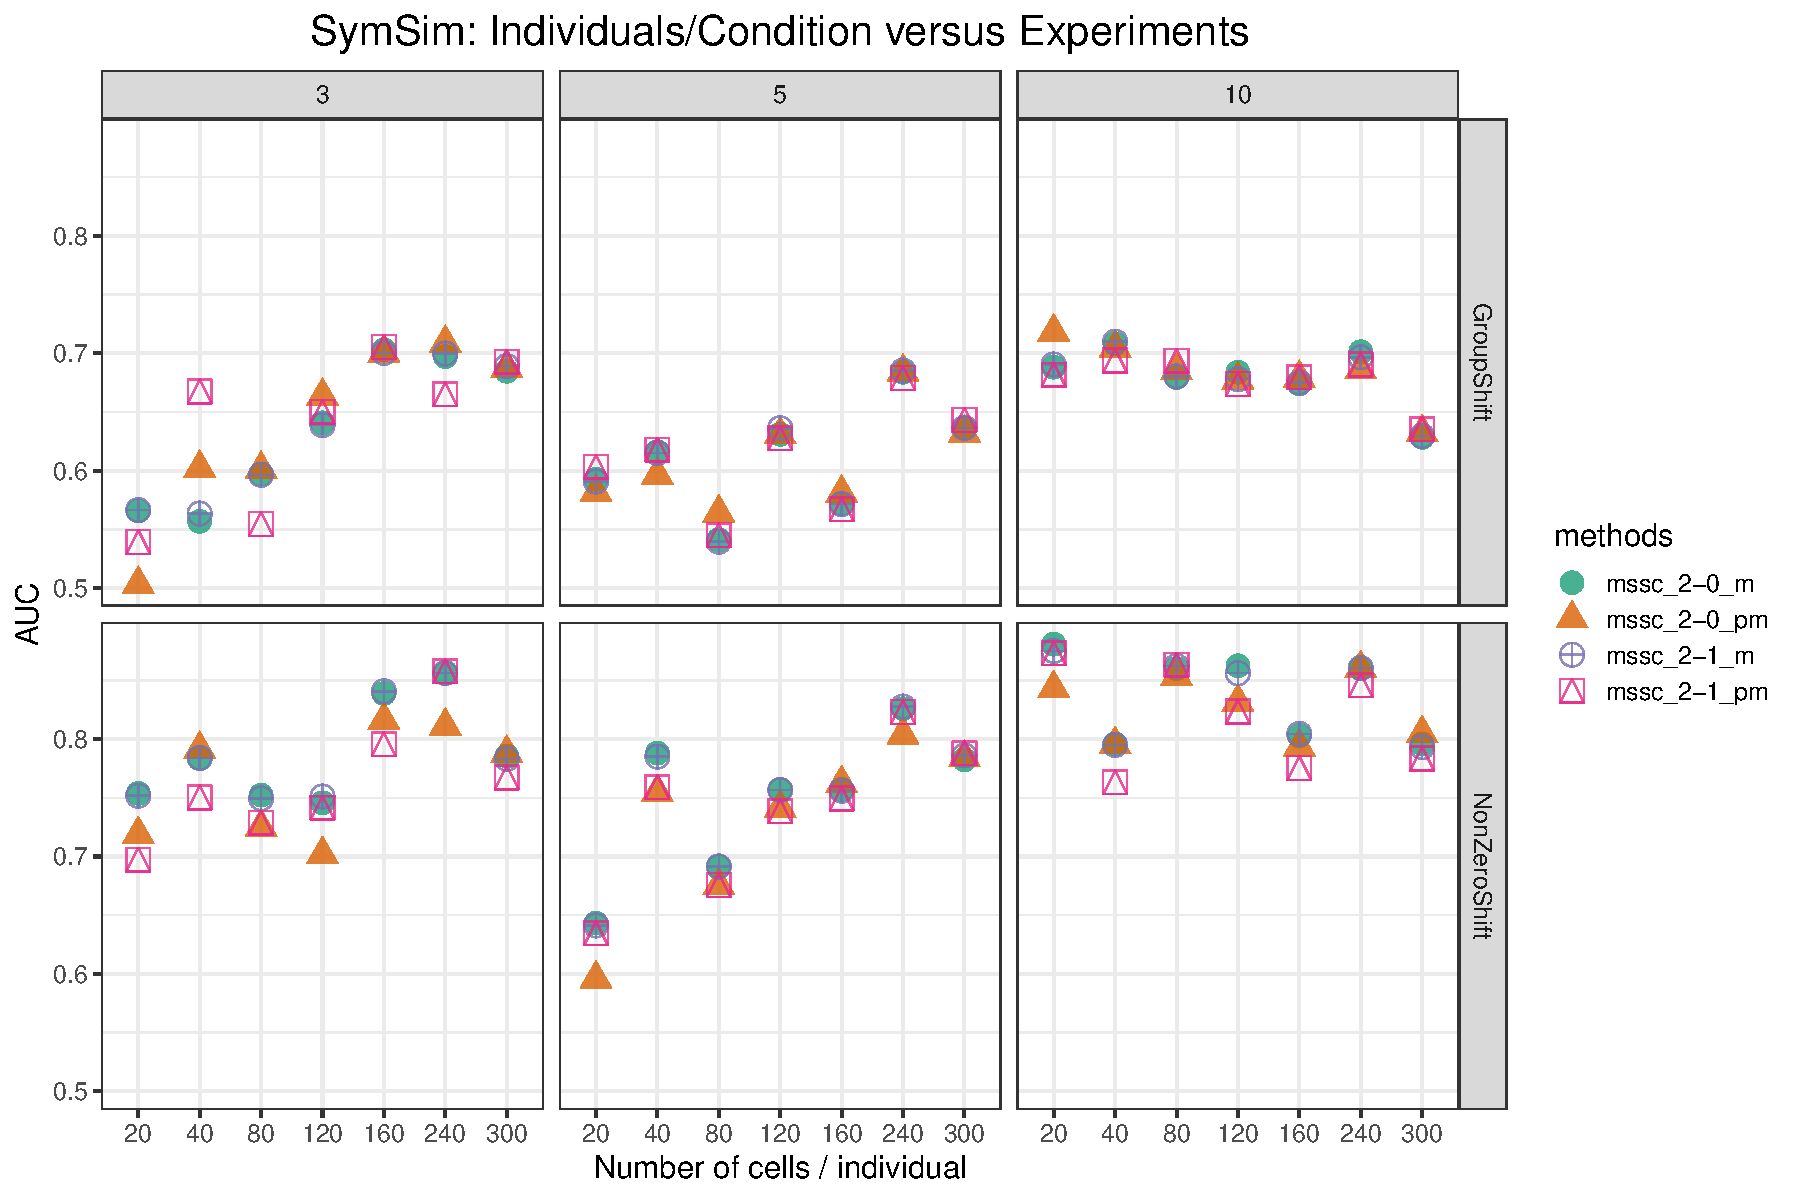
\includegraphics[width=\textwidth]{SymSim_mssc-20vs21_Summarize}
  \caption{Supplementary: comparing mssc20 and mssc21.}
\end{figure}

\section*{Method}
\subsection*{mssc}
We model the scRNA-Seq count data using Negative Binomial distribution. Let
\(y_i^{[g]}\) represent the count for the gene \(g\) in the cell \(i\), and \(j\)
is the individual the cell \(i\) belongs to. \(c_i\) is the condition under which
the cell \(i\) is treated.
\begin{align*}
  y_i^{[g]} &\sim NB(S_i\cdot\lambda_i^{[g]}, r^{[g]}) \\
  \log(\lambda_i^{[g]}) &= \mu^{[g]} + \mu_j^{[g]} + \mymucond^{[g]}
\end{align*}
\(S_i\) is the scaling factor for each cell. 
Here we set it as \(S_i = \frac{K_i}{{\it median}(\myvec{K})}\), where
\(K_i\) is the total count in the 
cell \(i\).\\

For each gene \(g\), we model the prior of \(\mu^{[g]}\) as a normal distribution. The hyper
parameters are shared among the genes.
\begin{align*}
  \mu^{[g]} &\sim \mathcal{N}(\mu_{\mathcal{G}}, \sigma^2_{\mathcal{G}}),~g=1,\dots,G\\
  \mu_{\mathcal{G}} &\sim \mathcal{I} \\
  \sigma^2_{\mathcal{G}} &\sim {\it Inverse Gamma} (\alpha_{\mathcal{G}}, \beta_{\mathcal{G}})
\end{align*}

For each gene \(g\), we model the prior of \(r^{[g]}\) as log-Normal distribution. The
hyper parameters are shared among the genes.
\begin{align*}
  log(r^{[g]}) &\sim \mathcal{N}(\mu_r, \sigma_r^2),~g=1,\dots,G\\
  \mu_r &\sim \mathcal{I} \\
  \sigma_r^2 &\sim {\it Inverse Gamma}(\alpha_r, \beta_r)
\end{align*}

For each gene \(g\) and each condition \(c\), we model the prior of \(\mymucond^{[g]}\) as a normal
distribution. The mean is zero, and the variance follows a Inverse Gamma
distribution, and is shared among the genes.
% TODO: how to distinguish between mu_c and mu_j?
\begin{align*}
  \mu_{c}^{[g]} &\sim \mathcal{N}(0, \sigma^2_{c}),~ g=1,\dots,G;~c=1,\dots,C\\
  \sigma_c^2 &\sim {\it Inverse Gamma}(\alpha_c, \beta_c),~c=1,\dots C,
\end{align*}

\mywarn{Mixture model as a prior for $\mu_{j}^{[g]}$, where $\sigma_0^2, \lambda_0$ are fixed.
\begin{align*}
  \mu_{c}^{[g]} &\sim (1 - \lambda_0)\mathcal{N}(0, \sigma^2_{1}) + \lambda_0 \mathcal{N}(0, \sigma^2_{0}),~ g=1,\dots,G;~c=1,\dots,C\\
  \sigma_1^2 &\sim {\it Inverse Gamma}(\alpha_1, \beta_1)
\end{align*}
}

For each individual \(j\), we model the prior of the individual effect
\(\mu_j^{[g]}\) as a normal distribution, whose mean \(\mu_j\) are shared among all the genes
for this particular individual. Then for different individuals, \(\mu_j\) have
the same prior of normal distribution, which is located at zero.

\mywarn{Maybe we can fix $\sigma_j^2$ or make it small.}
\begin{align*}
  \mu_j^{[g]} &\sim \mathcal{N}(\mu_j, \sigma_j^2),~g=1,\dots, G;~j=1,\dots, J \\
  \mu_j &\sim \mathcal{N}(0.0, \tau^2),~j=1,\dots,J\\
  \sigma_j^2 &\sim {\it Inverse Gamma}(\alpha_j, \beta_j),~j=1,\dots,J \\
  \tau^2 &\sim {\it Inverse Gamma}(\alpha_\tau, \beta_\tau)
\end{align*}

\subsection*{Model inference}
In total, we need to estimate about \(G\cdot(J + C + 2)\) parameters in mssc.
Generally, we have thousands of genes, around 10 or 20 individuals, and 2
conditions. In order to make mssc works efficiently in this scale, we apply the
variational inference to approximate the posterior distributions of these
parameters. And then use the samples from the approximated distributions for
further differential expression analysis.

\subsubsection{Mean-field variational inference}

Here we use the Automatic Differentiation Variational Inference (ADVI) provided
by Stan (a popular statistical programming language). A fully
factorized Gaussian distribution is used for the approximation. 

\begin{itemize}
\item
  The optimization target is to maximize the {\it Evidence lower
    bound} 
  (ELBO), which is defined as \(\mye_{q(\myvec{\theta})}\left(\log
    p(\myvec{y},\myvec{\theta}) - \log q(\myvec{\theta})\right)\).
  \(\myvec{\theta}\) are the stochastic variables defined above, such as
  \(\mu^{[g]}, \mu_c^{[g]}, \mu_j^{[g]}\) and so on. \(q_{\myvec{\phi}}(\cdot)\) is a fully
  factorized Gaussian distribution defined by the corresponding parameters
  \(\myvec{\phi}\).
\item
  For the stochastic variables like \(\sigma^2\), ADVI will use an one-to-one
  transformation to transform those variables into the unconstrained ones. So
  it's hard to have the analytic form for the approximated distributions of the
  original space, and the Monte Carlo sampling is used.
\item
  Reparameterization in the hierarchical model is important for variational
  inference.
\end{itemize}

Yao et al., 2018 estimates the performances of ADVI and shows the limitations of
variational inference. Here are some tips to use ADVI:
\begin{itemize}
\item
  The stopping rule is to increase ELBO into some stable points. But we should
  make it run furthermore. Here we set an extremely high criteria to let ADVI
  run for quite lots of steps.
\item
  Reduce the learning rate in ADVI. ADVI uses the modified version of AdaGrad as
  the optimizer, which could adjust the learning step for each parameters based
  on their gradients in each steps. But the
  scaling value of the learning step \(\eta\) tends to be over-estimated in the adaptive
  stage of ADVI. Here we fix it as 0.1.
\end{itemize}

\subsubsection*{Parameter initialization and hyper parameter estimation}
Parameter initialization is critical for variational inference. Here we use a
heuristic approach to initialize the parameters.
\begin{itemize}
\item \(\mu^{[g]}, r^{[g]}\) are firstly estimated by fitting the scaled Negative
  Binomial distribution.
\item
  \(\mu_c^{[g]}\) is estimated then using the sample mean minus the \(\mu^{[g]}\).
\item
  \(\mu_j^{[g]}\) is estimated similarly like \(\mu_c^{[g]}\).
\end{itemize}

Hyper parameters are estimated using the conjugate posterior formulation of the
corresponding parameters and their initial values estimated above.

\subsubsection*{Ranking statistics}
We use the ranking statistics \(\left|\mye_{q(\mu_{c1}^{[g]},
  \mu_{c2}^{[g]})}(\mu_{c_1}^{[g]}-\mu_{c_2}^{[g]})\right|\) to rank the genes for
differential expression analysis.

\subsection*{Simulation}
Secondly, we use a popular scRNA-Seq data simulation tool called SymSim (Zhang
et al., 2019) to evaluate our model. SymSim itself provides an
interface to add the batch effect directly to the observed counts, we
modify this function to support the simulation of the individual
effects.

\begin{itemize}
\item
  {\it Simulating the UMI-based scRNA-Seq data.} Parameters are set
  based on the suggestions in SymSim to simulate the UMI-based
  scRNA-Seq data. Specically, we set the protocol as "UMI", and the
  mean and variance of the sequencing depths, the number of PCR cycles
  are then chosen according the UMI-based parameters suggested by
  SymSim (See Supplementary for the details of the settings).
  
\item {\it Simulating the conditional expressions.} In order to
  simulate the scenarias that the cells are treated under different
  conditions, we treat different conditions as different
  cell populations in SymSim. Two conditions are considered here. The
  ground truth about the differential or non-differentia expressed genes
  is determined by SymSim. For each condition, we randomly partition the
  cells into different groups. Each group here corresponds to one
  individual.
\item
  {\it Simulating the individual effects.}
  We simulate the corresponding individual
  effects by modifying the way SymSim adds batch effect into
  different cells. Instead of adding the same batch effect for each
  condition in SymSim, here for each gene in each cell, we would
  simulate the corresponding individual effect, and then add that
  directly to the simulated count data generated by SymSim.

  We explore two kinds of simulating individual effect. One is to
  simulate same individual effects for different genes and cells
  in the same individual. The other one is simulate gene-specific
  individual effects.
  
  {\bf Simulating same individual effects for all the genes in the
    cells from one individual.}
  \begin{itemize}
    \item {\it Setting the individual effect size.} We firstly
      estimates the variations of the conditional expressions for
      a gene $g$, which is defined as
      $\Delta^{[g]} = |\mu_{c_1}^{[g]}-\mu_{c_2}^{[g]}|$. $c_1$ and $c_2$ are the index for
      two conditions. Then the individual effect is set as $\alpha
      \cdot Q_{0.975}(\myvec{\Delta}),~\myvec{\Delta} = \{\Delta^{[g]}:
      g=1, 2, ..., n_g\}$. $n_g$, the number of genes, is set as
      80. $\alpha$ is the scaling factor, which is set as 0.3 in our
      simulation. $Q_{0.975}(\cdot)$ is the quantile of
      0.975 for a given vector. $\mu_{c_1}^{[g]}$ and
      $\mu_{c_2}^{[g]}$ are estimated based on the heuristic approach
      used in estimating the initial values of them in our mssc model.
    \item {\it Choosing the individuals to add the individual
        effects.} We add the individual effects only to the chosen
      individuals. For the non-differential expressed genes, we
      randomly choose one condition and select part of the individuals
      randomly as 
      the candidate individuals, who would show strong individual
      effects for all these genes in the cells belonging to them. For
      the each of the differential expressed genes, we choose the
      condition where the gene shows relatively lower expressions. And
      then randomly choose part of the individuals in that conditions
      as the candidate individuals.
    \item
      {\it Adding the individual effects.} For each gene, we directly add the
      individual effects to all the cells for the candidate
      individuals. Two scenarias are further considered: a) {\it Group
        shift}: adding the individual effects to the cells even when the gene shows zero
      count in that cell; b) {\it Non-zero shift}: adding the
      individual effects to the cells when the gene shows at least one
      count in that cell.
    \end{itemize}
    {\bf Simulating gene-specific individual efffects.}
    \begin{itemize}
    \item
      {\it Setting the individual effect size and scale under the
        individual-level}. Let the common 
      individual effect size $\mu_b = \alpha
      \cdot Q_{0.975}(\myvec{\Delta})$, which follows the same
      definitions above. For an individual j, the corresponding
      individual effect size $\mu_j = \beta_j\cdot \mu_b$, where $\beta_j$
      will be fixed for individual j. For example, if we have three
      individuals in one condition, we would set $\beta_j, j = 1, 2,3$
      as $-1, 0, 1$. The same settings are followed for the rest of
      individuals in the other conditions.
      Let individual effect scale
      $\sigma_j = t \cdot \mu_j$, where t is chosen as 0.5.
    \item {\it Setting the individual effect for each gene.} For the
      gene g in the individual j, we set the specific individual
      effect $\mu_j^{[g]} \sim \mathcal{N}(\mu_j, \sigma_j^2)$.
    \end{itemize}
\end{itemize}

\bibliography{mssc_ref}

\section*{Acknowledgements (not compulsory)}
Acknowledgements should be brief, and should not include thanks to
anonymous referees and editors, or effusive comments. Grant or
contribution numbers may be acknowledged.

\section*{Author contributions statement}
Must include all authors, identified by initials, for example:
A.A. conceived the experiment(s), A.A. and B.A. conducted the
experiment(s), C.A. and D.A. analysed the results.  All authors
reviewed the manuscript.

\section*{Additional information}
To include, in this order: \textbf{Accession codes} (where
applicable); \textbf{Competing interests} (mandatory statement). The
corresponding author is responsible for submitting a
\href{http://www.nature.com/srep/policies/index.html#competing}{competing
interests statement} on behalf of all authors of the paper. This
statement must be included in the submitted article file.
\end{document}
